\label{sec:pers_recog}
As our robots need to operate and interact with people in a dynamic environment, our robots’ people detection skills have been upgraded. This skill is upgraded to a generalized system capable of recognizing people in 3D. In the people recognition stack, an RGB-D camera is used as the sensor to capture the scene information. A recognition sequence is completed in four steps. First, people are detected in the scene using OpenPose and if their faces are recognized as one of the learned faces in the robots'database, they are labeled using their known name using OpenFace. The detections from OpenPose are associated with the recognitions from OpenFace by maximizing the IoUs of the face ROIs. Then, for each of the recognized people, additional properties such as age, gender and the shirt color are identified. Furthermore, the pose keypoints of these recognitions are coupled with the depth information of the scene to re-project the recognized people to 3D as skeletons. Finally, information about the posture of each 3D skeleton is calculated using geometrical heuristics. This allows for the addition of properties such as “pointing pose” and additional flags such as `is\_waving', `is\_sitting', etc.
%The current design of our people recognition stack is loosely coupled. In the future, the design will be completely decoupled into the individual components, as most challenges do not require all the information generated by this system.
%
%\begin{figure}[H]
%	\centering
%    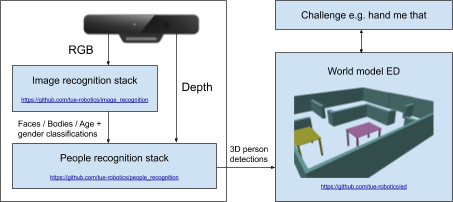
\includegraphics[width=0.7\linewidth]{pointing_pose}
%	\caption{The person detection pipeline}
%	\label{fig:people_recognition}
%\end{figure}